\subsection{Example}\label{sec:example}
As an example, let us consider a pipeline template $G^{\myLambda,\myGamma}$ as a sequence of three vertices modeling three key stages in our reference scenario: data preparation (\vi{1}), data enrichment (\vi{2}), and data storage (\vi{3}). Each stage is annotated with its policy set \P{i} and functional description \F{i}. Table~\ref{table:example} reports the policies and functional descriptions for each vertex, which are presented in the following.

%\begin{enumerate*}[label=n\arabic*)]
%  \item
The first vertex (\vi{1}) is responsible for data preparation.
It specifies an anonymization policy ($\myLambda(v_1)$) to protect sensitive information, such as personally identifiable information (PII) in the dataset.
The transformation function \TF{1} in $\myGamma(v_1)$ is an empty function \tf{a}, as no functional transformation is required for anonymization.
%   \item

The second vertex (\vi{2}) focuses on data enrichment, where additional information from the states of New York and New Hampshire is integrated into the dataset.
It requires a data enrichment policy ($\myLambda(v_2)$) to ensure that the added data are relevant and comply with privacy regulations.
The transformation function \TF{2} in $\myGamma(v_2$) is an additive function \tf{a}, which merges and integrates the external data with the existing dataset.
  %  \item

  The third vertex (\vi{3}) is responsible for aggregating data, including statistical measures like averages, medians, and some more statistics.
  It follows an aggregation policy ($\myLambda(v_3)$) to define how the aggregation should be performed, and ensure compliance with privacy and security regulations.
  The transformation function \TF{3} in $\myGamma(v_3)$ is a transformation function \tf{t}, which computes the required statistics and aggregates the data.
%\end{enumerate*}

\begin{figure}[ht!]
  \centering
  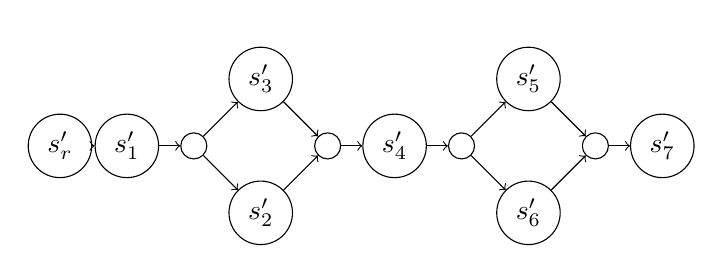
\begin{tikzpicture}[scale=0.85]
    \node[draw, circle] (node1) at (0,0) {$s^\prime_r$};
    \node[draw, circle] (node2) at (1,0) {$s^\prime_1$};
    \node[draw, circle] (node3) at (2,0) {$\timesOperator$};
    \node[draw, circle] (node4) at (3,-1) {$s^\prime_2$};
    \node[draw, circle] (node5) at (3,1) {$s^\prime_3$};
    \node[draw, circle] (node6) at (4,0) {$\timesOperator$};
    \node[draw, circle] (node65) at (5,0) {$s^\prime_4$};
    \node[draw, circle] (node7) at (6,0) {$\plusOperator$};
    \node[draw, circle] (node8) at (7,1) {$s^\prime_5$};
    \node[draw, circle] (node9) at (7,-1) {$s^\prime_6$};
    \node[draw, circle] (node10) at (8,0) {$\plusOperator$};
    \node[draw, circle] (node11) at (9,0) {$s^\prime_7$};
    % Text on top
    \node[above] at (node1.north) { \footnotesize$\instanceChartAnnotation$};
    \node[above] at (node2.north) { \footnotesize$\instanceChartAnnotation$};
    \node[above] at (node3.north) {};
    \node[above] at (node4.north) { \footnotesize$\instanceChartAnnotation$};
    \node[above] at (node5.north) { \footnotesize$\instanceChartAnnotation$};
    \node[above] at (node65.north) { \footnotesize$\instanceChartAnnotation$};
    \node[above] at (node8.north) { \footnotesize$\instanceChartAnnotation$};
    \node[above] at (node9.north) { \footnotesize$\instanceChartAnnotation$};
    \node[above] at (node11.north) { \footnotesize$\instanceChartAnnotation$};
    % Connection
    \draw[->] (node1) -- (node2);
    \draw[->] (node2) -- (node3);
    \draw[->] (node3) -- (node4);
    \draw[->] (node3) -- (node5);
    \draw[->] (node5) -- (node6);
    \draw[->] (node4) -- (node6);
    \draw[->] (node6) -- (node65);
    \draw[->] (node65) -- (node7);
    \draw[->] (node7) -- (node8);
    \draw[->] (node7) -- (node9);
    \draw[->] (node8) -- (node10);
    \draw[->] (node9) -- (node10);
    \draw[->] (node10) -- (node11);
  \end{tikzpicture}
  \caption{Service composition instance}
  \label{fig:service_composition_instance}
\end{figure}
